\chapter{Algorithm for test}
\label{cha:bacAlg}

In this chapter we present the bacteriological algorithm used to generate and
select the job configurations for Hadoop. 

\section{Genetic Algorithm}
\label{subsec:evolutionay_algorithms}
Evolutionary Algorithms are inspired of biological evolution process to select
the best inviduals that adapt themselves in the environment. For this adptation
are used some biological mechanisms such as reproduction, mutation, recombination
or crossover and \textbf{selection}. One of the most known evolutionary algorithms
is the Genetic Algorithm (GA). \nomenclature{$GA$}{- Genetic Algorithm}


On the context of GA there are three important components:
\begin{itemize}
    \item \textbf{Gene} that is the smallest particle.
    \item \textbf{Individual} that is composed of genes.
    \item \textbf{Population} that is composed of individuals.
\end{itemize}

The GA works at the gene level, so all changes are done at this level. At first
glance, changes done on gene seems tiny and irrelevant, but these chnages can
be crucial for adaptation of the individual in the environment. Genetic changes
can be crucial for the survival of one entire population or even mean survival
of a specie.

%Rosenzweig~\cite{rosenzweig:1995} cites that in the evolution
%process barriers may exist, like geographical barrier retricts gene flow within
%a sexually reproducing population and these genes could define the existence another
%population.

The GA process describes in~\ref{alg:ga} is based on tree biological
mechanisms: reproduction, crossover and mutation which are further detailed below:

\begin{itemize}
	\item \textbf{Reproduction}: copies the individuals to participe of the next
	stage (the crossover). They are chosen based on their ability to adapt the environment.
	Those abilities can be calculated according with a function \textit{F(x)} called
	the fitness of the individual.

    The choice of one individual is based in its fitness value. The choice process
	is similar to spin a roulette wheel where each individual receive slots according
    with its fitness, e.g. if an individual has F(X) = 10, then it has 10 slots
    in the roulette and suppose it has 100 slots, so the chance to choose this individual
    to participate in crossover is {\it100/F(X) = 1/10}. Thus the individual
    fitness is greater, then its number of copies tends to be greater.

	\item \textbf{Crossover}: the crossover is similar to the natural process called
	chromosomal crossover. This process is based on genetic recombination of
	chromosomes	to produce new genetic combinations. Basically the genes of two
    individuals are genetically combined to generate another resultant individual,
    so the new individual has some characteristics of both parents.
	More precisely, in the genetic algorithm two individuals are chosen randomly $(A, B)$,
	an integer k, between 0 and the size {\it n} of an individual minus one, is chosen
	randomly. The new individual $A'$ is composed by the first {\it k} genes of A
	and the last {\it k - n} genes of B. The individual $B'$ consists of the
	first {\it k} genes of B and the last {\it k - n} genes of A. 

	\item \textbf{Mutation}: is occurs after the crossover. One mutation occurs in the
	genes of new individuals. The natural process consists basically in change enzymes
    or proteins of genes in order to create new individuals. The mutation process
	of GA is simple, one or more genes are randomly selected and then are changed
    (e.g. change one or more nucleotides of the DNA	of one chromosome).

% or one gene is constituted for bits 0 or 1 and one bit is
%	changed from 0 to 1).
\end{itemize}

%\begin{figure}[htbp]
%	\centering
%	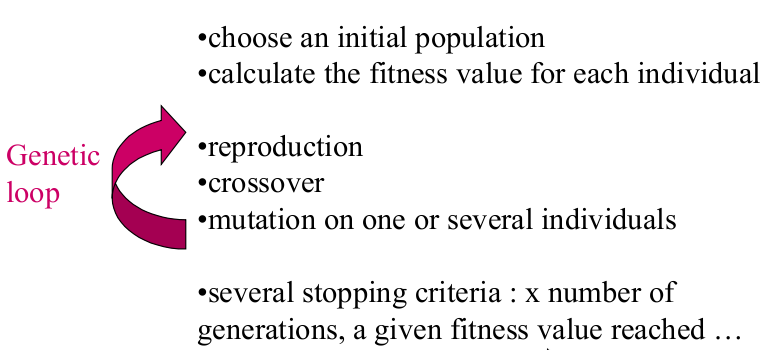
\includegraphics[width=\columnwidth]{img/ga.png}
%	\caption{Genetic Algotithm process - Figure extracted from~\cite{baudry}.}\label{fig:ga}
%\end{figure}

\begin{algorithm}
		\caption{Genetic Algorithm\label{alg:ga}}

        \SetKwInOut{Input}{Input}
        \SetKwInOut{Output}{Output}
		\Input{$Pop$ Initial population}
        \Output{$BestIndiv$ The best individual reached}

		\Repeat{X number of generations $\lor$ a give fitness value reached $\lor$ ...} {
			\For{\textbf{each} $indiv \in Pop$} {
				CalcFitness($indiv$)
			}

			Reproduction($Pop$)\\
			Crossover($Pop$)\\
			Mutation($Pop$)				

		}

		$BestIndiv \leftarrow getBestIndividual($Pop$)$
		
        \Return{$BestIndiv$}
\end{algorithm}

The algorithm starts with an initial population, for each individual is calculated
its fitness that is the base for reproduction mechanism, so the three biological
mechanisms are called in the specific order already detailed and so the resultant
population is evaluated as one or more criteria, if necessary the three mechanisms
are run again and the process continues until the criteria is achieved.

\section{Bacteriological Algorithm}

The Bacteriological Algorithm (BA) \nomenclature{$BA$}{- Bacteriological Algorithm}
is part of the family of genetic algorithms that
works on genetic context. A minor particle of this algorithm is a gene that influences
all phases of the algorithn. A group of genes forms an individual that have more
representativeness than an gene and a group of individuals forms one population.

Compared to GA the BA, the individual is a bacteria and the focus of the algorithm
is to adapt in a given environment.
%The BA is more one adaptive approach of GA than one otimization, 
The BA has some peculiarities to improve some issues involving the GA and change
it behavior.

The BAs introduces a new mechanism called memorization that is responsible for memorizing
the best individuals created along the generations. As described in~\cite{baudry},
it was proposed to improve the convergence of the GA, the introduction of the new
mechanism might appear a small modification, but actually reflects a crucial
change on GAs.

Besides, of the introduction of the new mechanism, the crossover mechanism was
removed because of the peculiar biological behavior of the bacterium. This mechanism
cannot be used anymore, in terms of natural bacteriologic process the remotion of
the crossover makes sense, the bacterium reproduce itself asexually, consequently
there is not crossover between two individuals, because the reproduction process
consists in duplicating the DNA of a bacterium and after a division to form two
new bacteria.

The algorithm in high-level of abstraction is described in~\ref{alg:ba}.
The BA is started and has four main mechanisms: Fitness computation, Memorization,
Reproduction and Mutation which are detailed below:

\begin{itemize}
	\item {\bf Fitness computation}: the fitness as in GA is one way to 	
	differentiate the abilities of each individual to adapt to the
	environment. Calculation depends on several criteria defined by 
	the programmer and is used to select the best individuals for the next generation.

	\item {\bf Memorization}: is the main mechanism introduced by the BAs. Its is responsible
	for memorizing the best individuals generated by the process of adaptation,
	as the process continues, the population improve more quickly its capacity of
	adaptation. The process consists in memorizing the best individuals through 
	the	generations, if one generation generates bad individuals, i.e. generate low
	fitness values, then the memorization operator ignores this generation and
	uses the best individuals from past generations to the next generation in order
	to avoid regressions in the process.

	\item {\bf Reproduction}: is similar to GA, the best individuals are sorted randomly
	and selected to the mutation process. One drawback in this stage is the population
    size may grow up exponentially, so thresholds must be established.

	\item {\bf Mutation}: is responsible for generating new individuals, one
	or several genes are changed in order to improve the adaptation of the bacteria
	population to the environment. These new individuals are evaluated by their
	fitness and they may be inserted in the set of best	individuals.

\end{itemize}


\begin{algorithm}
		\caption{Bacteriological Algotithm\label{alg:ba}}

        \SetKwInOut{Input}{Input}
        \SetKwInOut{Output}{Output}
		\Input{$Pop$ Initial population}
        \Output{$BestIndiv$ The best individual reached}

		$SetBestIndiv \leftarrow \{\}$

		\Repeat{X number of generations $\lor$ a give fitness value reached $\lor$ ...} {
			\For{\textbf{each} $indiv \in Pop$} {
				CalcFitness($indiv$)
			}
	
			SetBestIndiv.pop(Memorization($Pop$))\\
			Reproduction($Pop$)\\
			Mutation($Pop$)				

		}

		$BestIndiv \leftarrow getBestIndividual($SetBestIndiv$)$
		
        \Return{$BestIndiv$}
\end{algorithm}

%\begin{figure}[htbp]
%	\centering
%	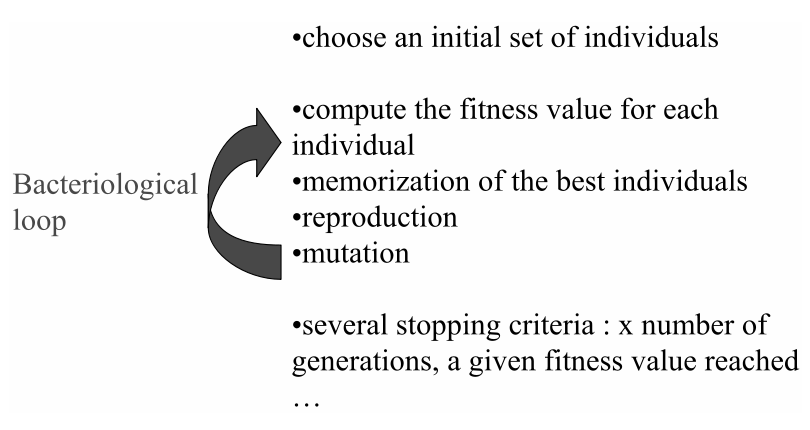
\includegraphics[width=\columnwidth]{img/ba.png}
%	\caption{Bacteriological Algotithm process - Figure extracted from~\cite{baudry}.}\label{fig:ba}
%\end{figure}

